\documentclass[12pt]{article}

\usepackage{sbc-template}
\usepackage{graphicx,url}
\usepackage[utf8]{inputenc}
\usepackage[T1]{fontenc}
\usepackage[brazil]{babel}
\usepackage{amsmath}

\sloppy

\title{Avaliação de Políticas de Substituição de Páginas:\\
  FIFO, OPT e LRU Aproximado}

\author{Pietro Mendes Prauchner\inst{1}}

\address{Universidade Federal do Pampa (UNIPAMPA) -- Campus Alegrete\\
  Alegrete -- RS -- Brasil
  \email{pietroprauchner.aluno@unipampa.edu.br}
}

\begin{document}

\maketitle

\begin{abstract}
  This paper compares the number of page faults produced by three page
  replacement policies --- FIFO, the optimal policy (OPT) and an approximate LRU
  based on a reference bit and an $N$-bit aging history --- over four real
  memory access traces of one million accesses each and their concatenation.
  The number of frames ranges from 4 to 64. The history width ($N=8$) and the
  aging interval ($I=100$ accesses) were chosen by an exploratory sweep. The
  approximate LRU had fewer faults than FIFO in every simulation, covering on
  average 36\% of the distance between FIFO and OPT, and proved far more
  sensitive to the aging interval than to the history width.
\end{abstract}

\begin{resumo}
  Este artigo compara o número de falhas de página de três políticas de
  substituição --- FIFO, a política ótima (OPT) e um LRU aproximado baseado em
  bit de referência e histórico de $N$ bits com envelhecimento --- sobre quatro
  traces reais de um milhão de acessos e sua concatenação, com 4 a 64 frames.
  A largura do histórico ($N=8$) e o intervalo de envelhecimento ($I=100$
  acessos) foram escolhidos por uma varredura exploratória. O LRU aproximado
  fez menos falhas que o FIFO em todas as simulações, cobrindo em média 36\% da
  distância entre o FIFO e o OPT, e mostrou-se muito mais sensível ao intervalo
  de envelhecimento do que à largura do histórico.
\end{resumo}

\section{Introdução}

Em um sistema com memória virtual paginada, o espaço de endereçamento de um
processo é dividido em páginas de tamanho fixo, e apenas parte delas ocupa
frames da memória física em cada instante. Quando um acesso referencia uma
página que não está em nenhum frame, ocorre uma \emph{falha de página}: o
sistema operacional precisa trazer a página do armazenamento secundário e, se
todos os frames estiverem ocupados, escolher uma \emph{vítima} para liberar
espaço~\cite{silberschatz:18}. Como cada falha custa ordens de grandeza mais
que um acesso à memória, a regra que escolhe a vítima --- a \emph{política de
substituição} --- tem impacto direto no desempenho.

Este trabalho avalia três políticas: FIFO, a política ótima de
Belady~\cite{belady:66} (OPT) e uma aproximação do LRU por envelhecimento
(\emph{aging})~\cite{tanenbaum:15}. Para isso, foi desenvolvido um simulador
que lê traces de acessos de programas reais e conta as falhas de página de
cada política variando o número de frames disponíveis. O objetivo é medir
quanto o LRU aproximado, que só depende de informação que o hardware fornece
de forma barata, se aproxima do limite inferior dado pelo OPT, e como seus dois
parâmetros --- a largura do histórico e o intervalo de envelhecimento ---
afetam esse resultado.

O restante do artigo está organizado assim: a Seção~\ref{sec:fundamentacao}
descreve as políticas; a Seção~\ref{sec:metodologia}, os traces, o simulador e
a escolha dos parâmetros; a Seção~\ref{sec:resultados} apresenta e discute os
resultados; e a Seção~\ref{sec:conclusao} conclui.

\section{Fundamentação}\label{sec:fundamentacao}

Em todas as políticas, o número de frames é fixo durante a simulação e todos
começam vazios. Enquanto há frame livre, a página que faltou simplesmente o
ocupa; a política só é consultada quando todos estão ocupados.

\subsection{FIFO}

A política FIFO (\emph{first in, first out}) escolhe como vítima a página
carregada há mais tempo, independentemente de quantas vezes ou quão
recentemente ela foi usada~\cite{silberschatz:18}. É simples de implementar ---
basta uma fila na ordem de carga ---, mas ignora a localidade: uma página muito
usada é expulsa assim que se torna a mais antiga. O FIFO também está sujeito à
anomalia de Belady, em que aumentar o número de frames pode aumentar o número
de falhas~\cite{tanenbaum:15}.

\subsection{OPT}

A política ótima, descrita por Belady~\cite{belady:66}, escolhe como vítima a
página cujo \emph{próximo uso} está mais distante no futuro --- ou que nunca
mais será usada. Ela produz o menor número de falhas possível para um dado
trace e número de frames, mas exige conhecer os acessos futuros, o que um
sistema real não pode fazer. Por isso serve de limite inferior: nenhuma
política implementável faz menos falhas que o OPT.

\subsection{LRU aproximado por envelhecimento}

O LRU (\emph{least recently used}) expulsa a página usada há mais tempo, apoiado
na localidade temporal: o passado recente é um bom preditor do futuro próximo.
Implementá-lo de forma exata exigiria registrar a ordem de todos os acessos, o
que é caro demais em hardware. O LRU aproximado usa, por página em frame, apenas
um \emph{bit de referência}, ligado pelo hardware a cada acesso, e um
\emph{histórico} de $N$ bits mantido pelo sistema
operacional~\cite{tanenbaum:15}.

A cada $I$ acessos (o \emph{intervalo de envelhecimento}), ocorre um
\emph{envelhecimento} de todas as páginas em frame: o histórico desloca um bit à
direita, o bit de referência entra como bit mais significativo e é então
desligado. Assim, o bit mais significativo do histórico representa o intervalo
mais recente, e lido como inteiro o histórico é maior quanto mais recente e
frequente foi o uso. Uma página recém-carregada começa com o bit de referência
ligado e o histórico zerado.

A vítima é escolhida em três critérios, nesta ordem: (i)~bit de referência
desligado; (ii)~menor histórico; (iii)~carregada há mais tempo (FIFO). O bit de
referência vem antes do histórico por ser a informação mais recente. Com a
ordem inversa, a página carregada desde o último envelhecimento, de histórico
zerado, seria sempre a próxima vítima, e a política ficaria pior que o FIFO. O
último critério garante que o desempate seja determinístico.

\section{Metodologia}\label{sec:metodologia}

\subsection{Traces}

Foram usados os traces disponibilizados pela UNIOESTE~\cite{traces:unioeste}.
Cada linha registra um acesso: um endereço de 32 bits em hexadecimal e o tipo
(\texttt{R} para leitura, \texttt{W} para escrita). Seguindo o enunciado, a
página tem 4096 bytes, de modo que o número da página é o endereço sem os 12
bits de deslocamento. Leituras e escritas contam igual, e as falhas
compulsórias --- o primeiro acesso a cada página --- entram na contagem.

A Tabela~\ref{tab:traces} resume os traces. Os quatro primeiros vêm de
programas distintos e são tratados como cargas independentes. O
\texttt{bigone} é \emph{exatamente} a concatenação \texttt{bzip}, \texttt{gcc},
\texttt{sixpack} e \texttt{swim}, nessa ordem (cada bloco de um milhão de
linhas é idêntico ao trace correspondente); ele não é um quinto programa, mas
foi mantido como uma carga com trocas de fase, em que o conjunto de páginas em
uso muda bruscamente três vezes.

\begin{table}[ht]
\centering
\caption{Traces utilizados}
\label{tab:traces}
\begin{tabular}{lrrr}
\hline
Trace & Acessos & Páginas distintas & Escritas \\
\hline
\texttt{bzip}    & 1.000.000 &   317 & 12,2\% \\
\texttt{gcc}     & 1.000.000 & 2.852 & 10,7\% \\
\texttt{sixpack} & 1.000.000 & 3.890 & 16,1\% \\
\texttt{swim}    & 1.000.000 & 2.543 &  6,7\% \\
\texttt{bigone}  & 4.000.000 & 8.254 & 11,4\% \\
\hline
\end{tabular}
\end{table}

\subsection{Simulador}

O simulador foi escrito em C++17, usando apenas a biblioteca padrão, e é
compilado com \texttt{g++ -O2}. Ele lê o trace uma vez para a memória, converte
cada endereço no número da página e roda uma simulação por número de frames,
emitindo uma linha de CSV por simulação. Cada política é uma função que recebe
a sequência de páginas e o número de frames (e, no LRU aproximado, $N$ e $I$) e
devolve o número de falhas:

\begin{itemize}
  \item \textbf{FIFO}: uma fila com a ordem de carga e um conjunto de hash das
    páginas residentes.
  \item \textbf{OPT}: o próximo uso de cada acesso é pré-calculado numa passada
    de trás para frente do trace; as páginas residentes ficam numa árvore
    ordenada por próximo uso, o que dá vítima em $O(\log k)$ para $k$ frames.
    É a única política que enxerga o futuro do trace.
  \item \textbf{LRU aproximado}: cada frame guarda página, bit de referência,
    histórico e posição de carga; a vítima é obtida por varredura linear dos
    frames, comparando a tupla (bit, histórico, posição de carga).
\end{itemize}

A simulação é determinística: não há aleatoriedade, e rodar a grade inteira
duas vezes gera arquivos CSV idênticos. Os gráficos foram gerados em Python com
\texttt{matplotlib} diretamente a partir dos CSV, sem nenhuma lógica de
simulação.

\subsection{Escolha de $N$, $I$ e dos números de frames}\label{sec:parametros}

O enunciado deixa a critério do aluno a largura do histórico ($N$), o intervalo
de envelhecimento ($I$) e os números de frames. Para escolher $N$ e $I$, foi
feita uma varredura exploratória sobre os quatro traces independentes. Como os
números absolutos de falhas variam muito entre traces, a métrica usada foi a
\emph{posição relativa} do LRU aproximado entre o OPT e o FIFO:
\begin{equation}
  p = \frac{F_{\mathrm{LRU}} - F_{\mathrm{OPT}}}{F_{\mathrm{FIFO}} - F_{\mathrm{OPT}}},
\end{equation}
em que $F$ é o número de falhas. Com $p=0$ o LRU aproximado iguala o ótimo; com
$p=1$, iguala o FIFO; acima de 1, é pior que o FIFO. A
Tabela~\ref{tab:varredura} mostra a média de $p$ sobre os frames de 4 a 64 e
sobre os quatro traces.

\begin{table}[ht]
\centering
\caption{Posição relativa média $p$ do LRU aproximado (0 = OPT, 1 = FIFO)
  por $N$ e $I$}
\label{tab:varredura}
\small
\begin{tabular}{c|ccccccccc}
\hline
$N \backslash I$ & 10 & 25 & 50 & 100 & 200 & 500 & 1000 & 10000 & 100000 \\
\hline
1  & 0,911 &       &       & 0,789 &       &       & 0,874 & 1,062 & 1,583 \\
2  & 0,883 &       &       & 0,715 &       &       & 0,784 & 0,994 & 1,584 \\
4  & 0,846 & 0,759 & 0,707 & 0,671 & 0,660 & 0,700 & 0,773 & 1,000 & 1,580 \\
8  & 0,774 & 0,704 & 0,663 & \textbf{0,638} & 0,640 & 0,694 & 0,769 & 1,000 & 1,579 \\
16 & 0,719 & 0,660 & 0,632 & 0,621 & 0,632 & 0,692 & 0,767 & 1,001 & 1,579 \\
32 & 0,673 &       &       & 0,612 &       &       & 0,765 & 1,000 & 1,579 \\
\hline
\end{tabular}
\end{table}

\textbf{Intervalo de envelhecimento: $I=100$ acessos.} Com $N=8$, é o melhor
intervalo da varredura ($I=200$ fica a 0,002). Os extremos ilustram o papel de
$I$. Um intervalo curto demais ($I=10$) faz a janela de memória do histórico,
da ordem de $N \cdot I$ acessos, ficar pequena: páginas usadas há pouco e há
muito tempo acabam com o mesmo histórico zerado, e o desempate recai no FIFO.
Um intervalo longo demais ($I \geq 10000$) deixa o bit de referência ligado em
quase todas as páginas, e a decisão passa ao histórico, em que as páginas
carregadas no intervalo corrente estão zeradas. A política então expulsa
justamente as páginas trazidas mais recentemente, chegando a $p \approx 1{,}58$,
pior que o FIFO.

\textbf{Largura do histórico: $N=8$ bits.} É onde o ganho satura: passar de 8
para 16 bits melhora $p$ em apenas 0,017, e de 8 para 32 em 0,026, ao custo de
dois a quatro bytes por página em vez de um. Oito bits cabem num byte, o que é
plausível num sistema real. Com $I=1000$, o ganho já satura em $N=4$, coerente
com a janela útil ser da ordem de $N \cdot I$ acessos.

\textbf{Números de frames: 4 a 64, passo 4 (16 pontos).} A faixa cobre o
``joelho'' do \texttt{bzip}, que com apenas 317 páginas distintas despenca de
falhas entre 8 e 12 frames, e a região em que as políticas mais diferem. Os
demais traces continuam caindo até 256 frames, mas, na varredura exploratória,
a razão entre LRU aproximado e FIFO se mantém estável acima de 64 frames, de
modo que estender a faixa não muda a conclusão.

Para os gráficos de sensibilidade, a grade final variou ainda
$I \in \{10, 100, 1000, 10000, 100000\}$ com $N=8$, e
$N \in \{1, 2, 4, 8, 16\}$ com $I=100$.

\section{Resultados}\label{sec:resultados}

\subsection{Comparação entre as políticas}

As Figuras~\ref{fig:falhas-indep} e~\ref{fig:falhas-bigone} mostram o número de
falhas de página em função do número de frames para as três políticas, com o
LRU aproximado em $N=8$ e $I=100$. A Tabela~\ref{tab:falhas} traz os valores
para uma seleção de números de frames.

\begin{figure}[ht]
\centering
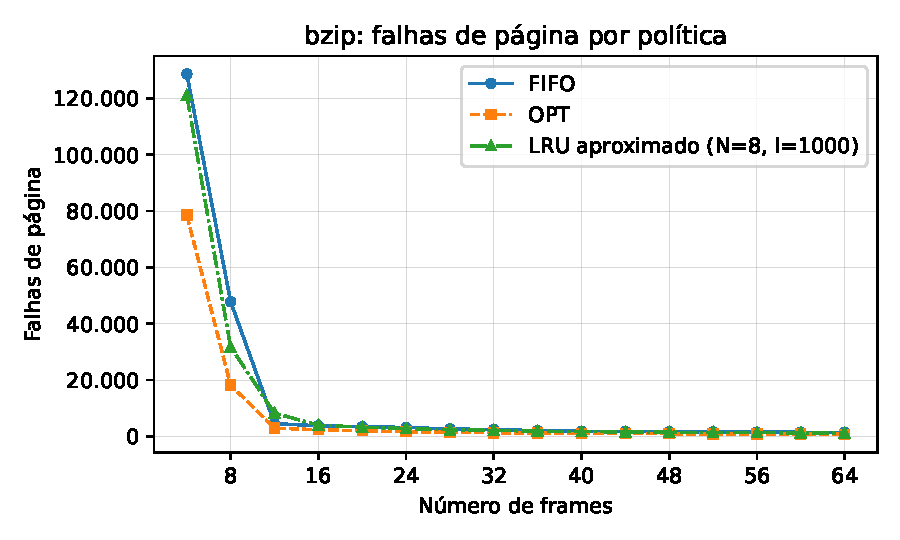
\includegraphics[width=.49\textwidth]{figuras/falhas_bzip.pdf}\hfill
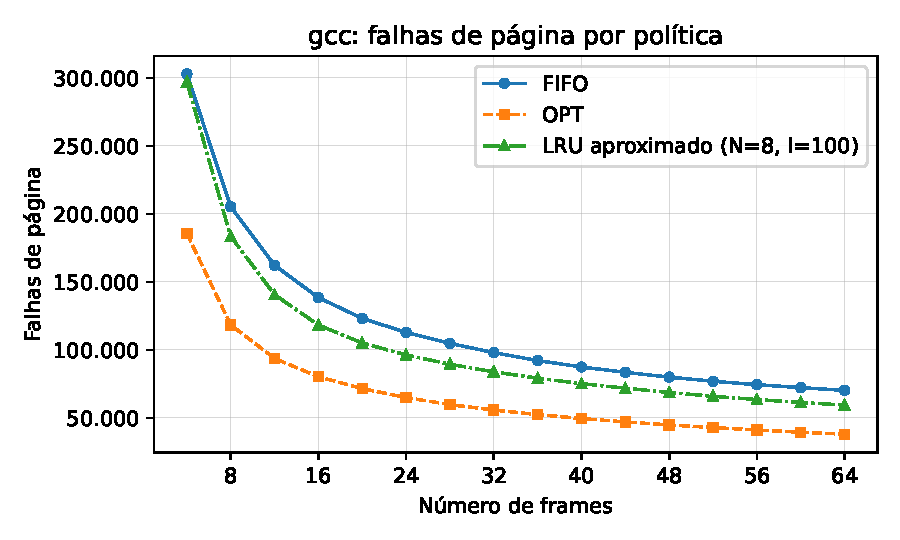
\includegraphics[width=.49\textwidth]{figuras/falhas_gcc.pdf}\\[2mm]
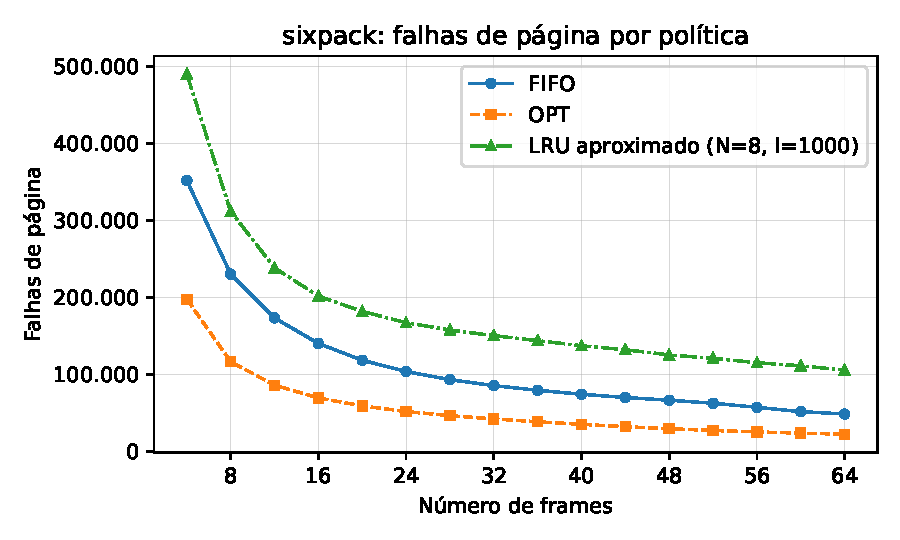
\includegraphics[width=.49\textwidth]{figuras/falhas_sixpack.pdf}\hfill
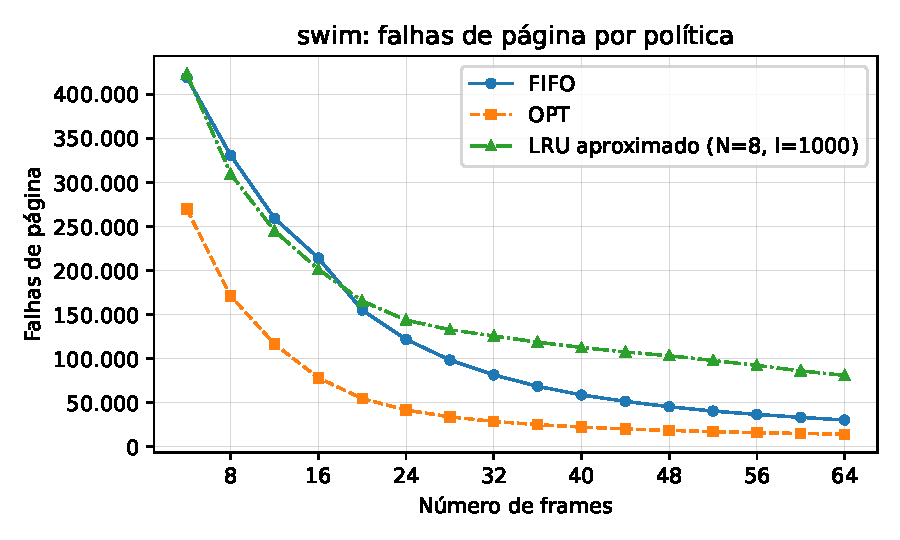
\includegraphics[width=.49\textwidth]{figuras/falhas_swim.pdf}
\caption{Falhas de página por número de frames nos quatro traces
  independentes, com LRU aproximado em $N=8$, $I=100$}
\label{fig:falhas-indep}
\end{figure}

\begin{figure}[ht]
\centering
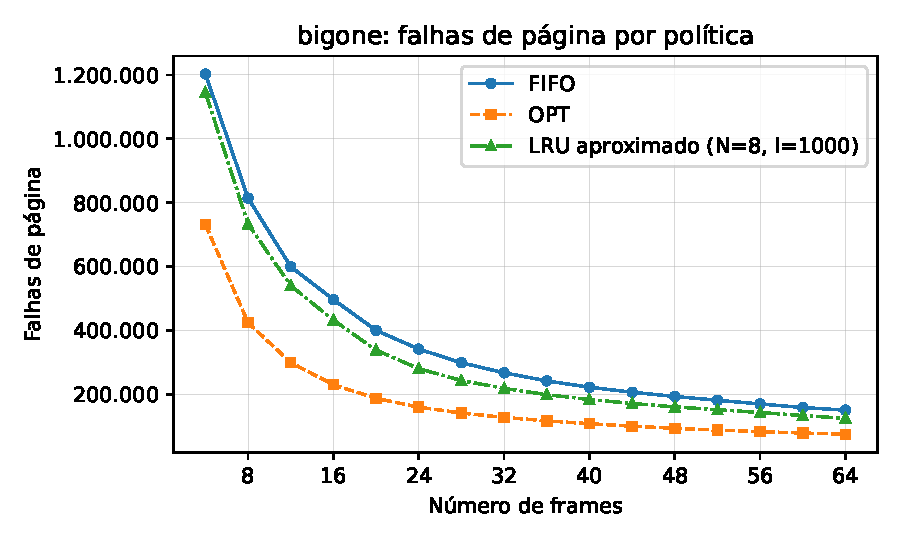
\includegraphics[width=.6\textwidth]{figuras/falhas_bigone.pdf}
\caption{Falhas de página por número de frames no \texttt{bigone}
  (concatenação dos quatro traces)}
\label{fig:falhas-bigone}
\end{figure}

\begin{table}[ht]
\centering
\caption{Falhas de página por política e número de frames (LRU aproximado com
  $N=8$, $I=100$)}
\label{tab:falhas}
\small
\begin{tabular}{llrrrrr}
\hline
Trace & Política & 4 & 8 & 16 & 32 & 64 \\
\hline
\texttt{bzip}    & FIFO & 128.601 &  47.828 &   3.820 &   2.497 &   1.467 \\
                 & LRU aprox. & 112.197 &  29.205 &   3.430 &   2.257 &   1.387 \\
                 & OPT  &  78.562 &  18.251 &   2.427 &   1.330 &     821 \\
\hline
\texttt{gcc}     & FIFO & 302.860 & 205.368 & 138.539 &  98.067 &  70.315 \\
                 & LRU aprox. & 297.010 & 183.514 & 118.351 &  83.924 &  59.484 \\
                 & OPT  & 185.754 & 118.480 &  80.307 &  55.802 &  38.050 \\
\hline
\texttt{sixpack} & FIFO & 351.810 & 230.168 & 140.083 &  85.283 &  48.301 \\
                 & LRU aprox. & 270.706 & 178.770 & 107.976 &  66.826 &  42.019 \\
                 & OPT  & 197.551 & 116.407 &  69.325 &  41.955 &  22.083 \\
\hline
\texttt{swim}    & FIFO & 419.509 & 330.893 & 214.295 &  81.638 &  30.422 \\
                 & LRU aprox. & 348.046 & 278.376 & 159.820 &  47.214 &  23.139 \\
                 & OPT  & 270.046 & 171.244 &  78.312 &  28.826 &  14.289 \\
\hline
\texttt{bigone}  & FIFO & 1.202.780 & 814.257 & 496.736 & 267.469 & 150.507 \\
                 & LRU aprox. & 1.027.959 & 669.865 & 389.577 & 200.219 & 126.027 \\
                 & OPT  &   731.913 & 424.381 & 230.369 & 127.910 &  75.228 \\
\hline
\end{tabular}
\end{table}

Em todas as 80 combinações de trace e número de frames, a ordem esperada se
manteve: o OPT fez menos falhas que o LRU aproximado, que por sua vez fez menos
que o FIFO. O número de falhas do FIFO também caiu monotonicamente com o número
de frames em todos os traces, ou seja, a anomalia de Belady não apareceu nos
pontos avaliados.

A Tabela~\ref{tab:resumo} quantifica a diferença, em média sobre os 16 números
de frames. O OPT reduz as falhas do FIFO em 43\% a 58\%, conforme o trace; o
LRU aproximado recupera parte desse ganho, de 10\% (\texttt{bzip}) a 32\%
(\texttt{swim}). Na média dos quatro traces independentes, a posição relativa
é $p = 0{,}638$: o LRU aproximado percorre cerca de 36\% da distância entre o
FIFO e o ótimo.

\begin{table}[ht]
\centering
\caption{Redução média de falhas em relação ao FIFO e posição relativa $p$ do
  LRU aproximado, sobre os frames de 4 a 64}
\label{tab:resumo}
\begin{tabular}{lrrr}
\hline
Trace & LRU aprox. vs.\ FIFO & OPT vs.\ FIFO & $p$ \\
\hline
\texttt{bzip}    & $-$10,0\% & $-$43,0\% & 0,778 \\
\texttt{gcc}     & $-$13,4\% & $-$43,1\% & 0,691 \\
\texttt{sixpack} & $-$19,5\% & $-$52,0\% & 0,620 \\
\texttt{swim}    & $-$31,6\% & $-$58,1\% & 0,464 \\
\texttt{bigone}  & $-$20,8\% & $-$50,7\% & 0,591 \\
\hline
\end{tabular}
\end{table}

O comportamento varia com o trace. No \texttt{bzip}, que usa só 317 páginas, as
três curvas despencam entre 8 e 12 frames e depois quase se sobrepõem: com 16
frames ou mais, o conjunto de páginas em uso a cada momento cabe quase todo na
memória, e as falhas ficam na casa de poucos milhares para as três políticas
(o mínimo possível são as 317 compulsórias). A diferença entre as políticas se concentra nos números de
frames pequenos --- com 8 frames, o LRU aproximado faz 39\% menos falhas que o
FIFO. No \texttt{swim}, o ganho do LRU aproximado é o maior: passa de 40\%
entre 24 e 36 frames, com pico de 43\% em 28 frames: o programa reutiliza com frequência um conjunto de páginas
que o FIFO expulsa por idade e o histórico preserva. No \texttt{gcc} ocorre o
oposto: com 4 frames o LRU aproximado quase empata com o FIFO ($-$1,9\%), pois
há tão poucos frames que quase todas as páginas residentes estão em uso em
cada intervalo e o histórico pouco as distingue.

No \texttt{bigone}, a posição relativa ($p=0{,}591$) é próxima da média dos
quatro traces que o compõem, o que é esperado, já que as trocas de fase são
apenas três em quatro milhões de acessos.

\subsection{Sensibilidade a $I$ e $N$}

A Figura~\ref{fig:sensibilidade} mostra, para o \texttt{bigone}, o efeito de
variar $I$ com $N=8$ e de variar $N$ com $I=100$. Os gráficos dos demais traces
seguem o mesmo padrão.

\begin{figure}[ht]
\centering
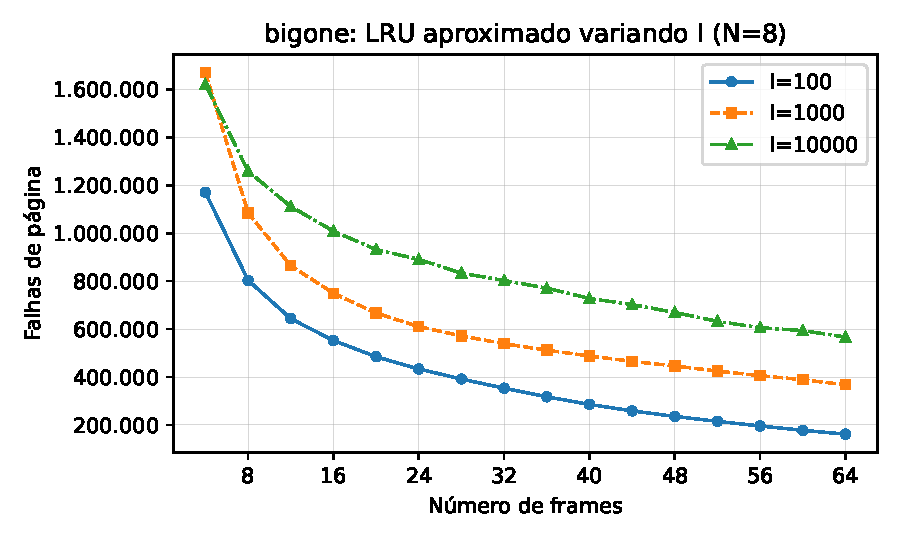
\includegraphics[width=.49\textwidth]{figuras/sensibilidade_i_bigone.pdf}\hfill
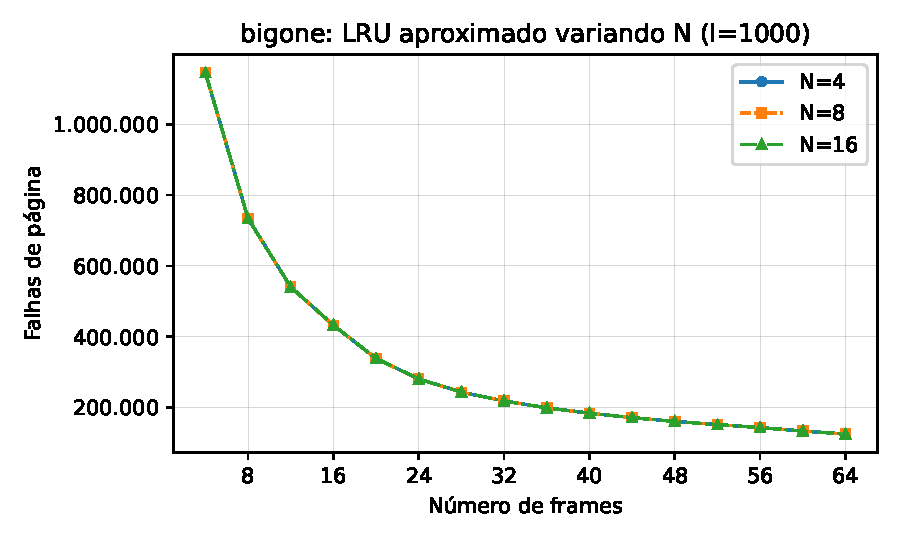
\includegraphics[width=.49\textwidth]{figuras/sensibilidade_n_bigone.pdf}
\caption{Sensibilidade do LRU aproximado no \texttt{bigone}: variando $I$ com
  $N=8$ (esquerda) e variando $N$ com $I=100$ (direita)}
\label{fig:sensibilidade}
\end{figure}

O intervalo de envelhecimento é, de longe, o parâmetro mais influente. Com
$I=100000$, o LRU aproximado chega a ser pior que o FIFO: no \texttt{bzip} com
12 frames, faz 27.641 falhas contra 4.581 do FIFO e 4.023 do par de referência,
pelo mecanismo descrito na Seção~\ref{sec:parametros}. Mesmo $I=1000$, que à
primeira vista parece razoável, fica pior que o FIFO em alguns pontos (8.303
falhas no \texttt{bzip} com 12 frames; 352.883 contra 302.860 no \texttt{gcc}
com 4 frames). Já $I=10$ é a melhor escolha com 4 frames em todos os traces, mas perde para $I=100$ à medida que o número de frames cresce, quando
uma janela de memória mais longa passa a ser útil.

A largura do histórico pesa bem menos. Com $I=100$ e até 16 frames, as curvas
de $N=2$ a $N=16$ diferem em menos de 1\%; só $N=1$ se destaca (até 19\% mais
falhas que $N=8$, no \texttt{swim}), por reduzir o histórico a ``usada ou não
no último intervalo''. Com mais frames, um histórico mais longo passa a valer:
com 64 frames, $N=4$ faz de 1,5\% a 5,8\% mais falhas que $N=8$, e $N=16$, de
1,1\% a 5,5\% menos, conforme o trace.

\section{Conclusão}\label{sec:conclusao}

Este trabalho comparou, por simulação sobre traces reais, o número de falhas de
página das políticas FIFO, OPT e LRU aproximado por envelhecimento. O LRU
aproximado, com histórico de 8 bits e envelhecimento a cada 100 acessos, fez
menos falhas que o FIFO em todas as 80 combinações de trace e número de frames,
reduzindo as falhas em 10\% a 32\% na média de cada trace e percorrendo cerca de
36\% da distância entre o FIFO e o ótimo. O OPT, inalcançável na prática,
mostra que ainda há margem considerável: ele faz de 43\% a 58\% menos falhas
que o FIFO.

O principal aprendizado sobre o LRU aproximado é que seu desempenho depende
muito mais do intervalo de envelhecimento do que da largura do histórico. Um
intervalo mal escolhido --- longo demais --- torna a política pior que o FIFO,
enquanto aumentar o histórico além de 8 bits traz ganhos marginais. A ordem
dos critérios de escolha da vítima também se mostrou essencial: consultar o
bit de referência antes do histórico evita que as páginas recém-carregadas
sejam sempre as primeiras expulsas.

Como trabalhos futuros, cabe comparar o LRU aproximado com o LRU exato e com o
algoritmo do relógio (segunda chance), avaliar o efeito de distinguir páginas
modificadas (o custo de escrita de volta, ignorado aqui) e ajustar $I$ de forma
adaptativa ao número de frames.

\bibliographystyle{sbc}
\bibliography{referencias}

\end{document}
